\documentclass[11pt,twoside,a4paper]{article}
\usepackage[utf8]{inputenc}
\usepackage[czech]{babel}
\usepackage{url}
%\usepackage{stdpage}
\usepackage[pdftex]{graphicx}
\usepackage{wrapfig}
\usepackage[pdftitle={Moderní firewally},pdfauthor={Pavel Benáček},
bookmarks=true,colorlinks=true,unicode=true]{hyperref}

%nastaveni normostrany
\hoffset -1.54cm
\voffset -0.04pt
\evensidemargin 1.5cm
\oddsidemargin 2.5cm
\topmargin -1.6cm
%%% Vyska textu 237 mm
%%% Sirka textu 150 mm
\textheight 237mm
\textwidth 150mm

\title{Moderní firewally}
\author{Pavel Benáček}

\begin{document}

\maketitle

\begin{abstract}

V dnešní době začíná být vnímána počítačová bezpečnost velmi vážně. Internet je decentralizovana síť, ve které na nás čekají různá nebezpečí. Bezpečnost je proto velice důležitým tématem, protože tuto síť potřebujeme pro naší každodenní práci (vyhledávání informací, elektronická pošta, práce na dálku přez zabezpečené SSH spojení a další). Mezi základní obranou linii patří prvek zvaný \underline{firewall}. O tomto základním prvků pojednává tento dokument. Popíše základní typy firewallů se zaměřením na modernější verze. Také uvede určité základní nástroje, které se dají pro tvoření firewallů použít.
\end{abstract}

\tableofcontents

\section{Úvod}

Firewall patří mezi základní bezpečnostní mechanismy při výstavbě moderních počítacových sítí. Jeho základním úkolem je provádění filtrace síťového provozu a to jak odchozího, tak i příchozího. Z hlediska bezpečnosti je důležité filtraci a inspekci paketů provádět v obou směrech. Častým omylem je to, že je hlavní inspekce a filtrace provozu prováděna pouze v příchozím směru. Toutu metodou můžeme profiltrovat velkou část nebezpečného provozu v průběhu útoku (například DoS, scan portů ..). Stejně nebezpečný je však i odchozí provoz, kdy může útočník realizovat validní spojení do Internetu, po kterém může být realizován samotný útok do samotného nitra chráněné síťe.

\textbf{TODO -- sepsat obsah částí}
 
\section{Základní popis a klasifikace}\label{sec:defend} 

Jak již bylo řečeno, firewall slouží jako základní prvek pro filtraci paketů. A to v jak odchozím, tak i příchozím směru.

Obecně by mohl být firewall definován jako síťové zařízení, které slouží k řízení a zabezpečení síťového provozu mezi síťemi s různou důvěryhodností a zabezpečením. Zjednodušeně se dá říci, že se jedná o bod v síti, kde jsou definována pravidla (ať již omezující nebo povolující) pro komunikaci mezi síťěmi, které se takto oddělují. Základní umístění v síti je naznačeno na obrázku \ref{pic:firewall_base}. Zde je filtrování prováděno mezi naší lokální LAN(local area network) sítí a externí WAN(wide area network) sítí

\begin{figure}[ht]
	\center
	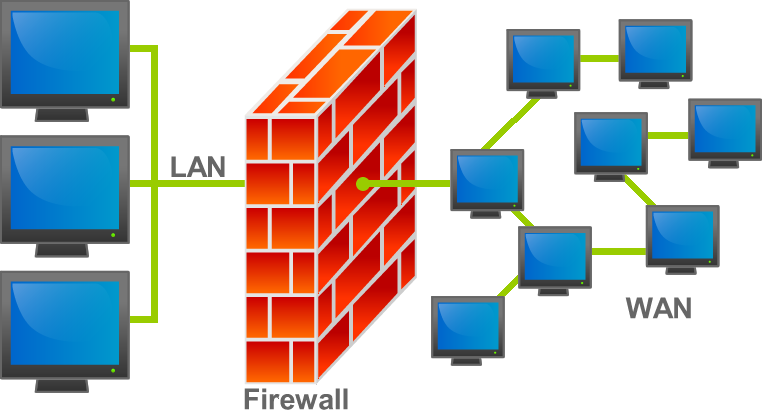
\includegraphics[scale=0.3]{./pict/firewall.png}
	\label{pic:firewall_base}
	\caption{Základní umístění firewallu}
\end{figure}

Firewally můžeme klasifikovat pomocí různých kriterií. Mezi základní však patří:
\begin{itemize}
	\item Dle realizce (softwarové a hardwarové)
	\item Dle síťové vrstvy, na které provádí inspekci (paketové filtry, stavové firewally, aplikační brány ..)
\end{itemize} 

Jejich podrobnější popis bude uveden v částech dále následujících.

\subsection{Dělení dle realizace}
Zde rozeznáváme dvě kategorie. První kategorií je softwarová realizace a druhou kategorií je hardwarová realizace. Softwarová realizace firewallu patří mezi nejpoužívanější. Mezi její veliké výhody patří jejich přívětivá cena a dostupnost. Navíc není většinou nutné kupovat specializovaný hardware a jsou velice konfiguravatelné. Takovýto softwarový firewall můžeme vytvořit bez větších nákladů pomocí nástoje iptables, který je součástí každé serverové(ale v dnešní době i klientské) linuxové distribuce. Takto vytvořený firewall může však být pro začínajícího administrátora docela komplikovaný, proto je dobré šáhnou i po placených firewallech třetích stran.

Mezi základní a nespornou vlastnost hardwarových firewallů patří jejich rychlost. Obsahují totiž hardware, který je navrhnut pro samotnou činnost firewallu. Jejich výměna za modernější verzi je však více nákladná.

\subsection{Dělení dle síťové vrstvy}

\begin{figure}
	\center
	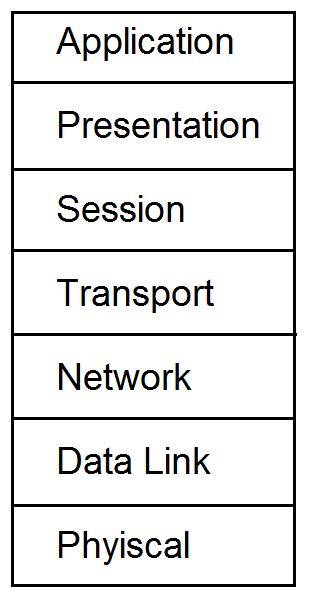
\includegraphics[scale=0.25]{./pict/osi.png}
	\label{pic:osi_model}
	\caption{ISO/OSI model}
\end{figure}

V síťové oblasti se základní funkce dělí do takzvaných vrstev. Jeden z nejpoužívanější je ISO/OSI model. Tento model dělí síťovou komunikaci na sedm vrstev. Nebudu se zde podrobně věnovat popisu jednotlivých vrstev, ale pro pochopení problému filtrace je důležitý aspoň základní popis. ISO/OSI model je naznačen na obrázku \ref{pic:osi_model}. Firewally většinou pracují od vrstvy 3 do vrstvy 7. 


Vrstva 3 je vrstva, kam se řadí protokol IP. Zde může být prováděna filtrace na základě IP adresy. Hodně často se však požaduje i filtrace podle takzvaných portů. Porty definuje vrstva číslo 4. Protokoly, které pracují na této vrstvě jsou TCP (Transmission Control Protocol) a UDP(User Datagram Protocol). 

Pro větší bezpečnost provozu se však provádí kontrola i na vrstvě číslo 7. Firewally, které pracují na této vrstvě patří mezi nejnovější a nejbezpečnější produkty v oblasti bezpečnosti. Jejich síla tkví v tom, že dokážou rozeznat protokol, který se v daném paketu přenáší. Může tedy pokrýt i ty případy, kdy se útočník snaží zakázaný protokol přesměrovat na svůj port, který je však v pravidlech firewallu povolen(například port 53 - služba DNS).

Pomocí tohoto popisu můžeme rozdělit firewally do několika základních kategorií:
\begin{itemize}
	\item Paketové filtry
	\item Stavové paketové filtry
	\item Aplikační brány
	\item Stavové paketové filtry s kontrolou protokolů a IDS
\end{itemize} 

\subsection{Paketové filtry}
Patří mezi nejstarší formu firewallu. Provádí základní filtraci provozu na vrstvě 3(IP) a 4(TCP/UDP). Výhodou je rychlost a jednoduchost konfigurace. Nevýhodou je nízká úroveň kontroly procházejících spojení. Mezi typické představitele patří nástroj iptables nebo ACL(Access Control Lists) v systému IOS od routerů společnosti Cisco.

\subsection{Stavové paketové filtry}
Tyto firewally provádějí kontrolu stejně jako paketové filtry, navíc si však ukládají informace o povolených spojeních. Například, jestli bylo navázáno spojení pro určitou komunikaci. Pakety, které patří do daného povoleného spojení pak nemusí procházet procesem kontroly a mohou být rovnou povoleny. Stavová inspecke má tedy dvě výhody. První výhodou je urychlení filtrace paketů k již navázanému spojení. Takové pakety nemusí procházet celým rozhodovacím procesem. Druhou výhodou je to, že i když povolíme pouze odchozí směr, tak firewall nám sám povolí příchozí validní komunikaci. Můžeme tak například nastavit jedno pravidlo pro FTP protokol pro odchozí komunikaci a firewall sám povolí porty nutné k úspěšné komunikaci po FTP.

Mezi velké výhody paketových filtrů patří jejich vysoká rychlost, poměrně slušná úroveň zabezpečení a jednodužší konfigurace, která snižuje pravděpodobnost případné chyby v konfiguraci. Oproti aplikačním branám poskytují nižší zabezpečení. Představitelé této kategorie je opět iptables v Linuxu, ipfw v systémech *BSD,starší verze Cisco PIX a Cisco IOS Firewall.

\subsection{Aplikační brány}
Aplikační brány jsou známé i pod názvem proxy firewally. Veškerý provoz ze sítě prochází přez tento bod formou dvou spojení. Klient(též zvaný iniciátor) se připojí na proxy server, ten příchozí spojení zpracuje a na základě tohoto požadavku vytvoří spojení na cílový server (v roli aplikačního klienta). Data, která dostane od serveru, poté přepošle klientovi. Kontrola se provádí na aplikační vrstvě (vrstva číslo 7).

Vedlejším efektem je to, že server nevidí cílovou adresu klienta, ale adresu proxy serveru. Brány tak automaticky působí jako NAT(Network Address Translation). Funkci NATu mají však i routery a jiné zařízení. Velkou výhodou je bohatá možnost konfigurace, která se zde nabízí. Proxy totiž může nahlédnout do samotného provozu na nejvyšší vrstvě. Získá tak mnohem více informací než paketový filtr nebo stavový paketový filtr.

Nevýhodou je však náročnost na potřebný hardware. Aplikační brány jsou schopny zpracovat mnohonásobně nižsí počet spojení a rychlosti, než paketové filtry. Dalším nepříjemným jevem jsou větší latence.  

I přez tyto nevýhody je tento druh firewallu velice bezpečným a umožňuje dostatečně nakonfigurovat i podrobná pravidla. Bezesporu se jedná o jednoho ze zástupců moderních firewallů. Představitelé této kategorie jsou například The~Firewall~Toolkit~(fwtk) a z něj vycházející Gauntlet.

\subsection{Stavové paketové filtry s kontrolou protokolů a IDS}
Tento druh firewallů si kromě informaci o stavu, schopnosti dynamicky otevírat porty pro různá řídící a datová spojení přináší něco, co se označuje jako \textit{Deep inspection} nebo \textit{Application Intelligence}. Firewally jsou schopny kontrolovat procházející spojení až na datovou úroveň známých protokolů i aplikací. Mohou tak zakazovat například průchod FTP spojení, v němž se objeví indikátory, že se nejedná o FTP spojení, ale tunelování jiného protokolu. Tuto metodu tunelování často využívají P2P sítě(Torrenty, Gnutella, Napster, atd.) Dalším indikátorem může například být nesprávný formát emailové hlavičky. 

Nejnověji se do  těchto druhů firewallů implementují takzvané IDS(Intruder Detection System). Jedná se o systém pro detekci útoků, které pracují podobně jako antiviry. V datovém toku vyhledávají pomocí různých heuristických analýz známé vzory, které naznačují možnost útoku. Díky heuristické funkce jsou schopny reagovat i na modifikované typy útoků. Útočníci si ale dávají pozor, aby novější útok nebyl detekovatelný nejnovějšími IDS systémy (a nebo byl aspoň složitěji detekovatelný). Mohou odhalit vzorce útoků i ve zdánlivě nesouvisejících pokusech o spojení, např. skenování adresního rozsahu, rozsahu portů, známé signatury útoků uvnitř povolených spojení a další.

Výhodou těchto systémů je vysoká úroveň bezpečnosti, relativně snadná konfigurace a docela vysoká rychlost inspekce toku. Jsou však pomalejší než stavové paketové filtry.

Nevýhodou je to, že tyto moderní firewally integrují obrovské množství funkcionality a je tak zvýšena pravděpodobnost zneužitelné chyby (nikdo není dokonalý :-), díky které se může útočník dostat do chráněné sítě.

Mezi typické představitele patří produkty řady Netscreen, ISG a SSG společnosti Juniper. Podobnou funkcionalitu nabízi i iptables, který je dostupný v Linuxových distribucích. 

\section{IDS a IPS systémy}
Dnešní moderní firewally velice často spolupracují s takzvanými systémy IDS(Intrusion Detection System) a IPS(Intrusion Prevention System).

\end{document}

